\chapter{Witten Diagrams and Mellin Amplitudes}
\label{ch:volume-iii-witten-diagrams-mellin-amplitudes}

\section{Tree-Level Diagrams for Correlators}

The generating functional
\[
  Z_{\rm bulk}[\varphi_0]
  =
  \left\langle
    \exp\left(\int\dd^Dx\,\varphi_0(x)\mathcal O(x)\right)
  \right\rangle
\]
turns classical bulk perturbation theory into a diagrammatic expansion of
CFT correlation functions.  A Witten diagram is a bulk Feynman diagram whose
external legs end on specified boundary insertion points.  Internal vertices
are integrated over \(\mathrm{AdS}_{D+1}\) with the invariant measure
\[
  \dd^{D+1}X\,\sqrt g
  =
  R^{D+1}\frac{\dd^Dx\,\dd z}{z^{D+1}}
\]
in the upper half-space coordinates.

For a cubic scalar interaction
\[
  S_{\rm int}
  =
  \int\dd^{D+1}X\,\sqrt g\,
  g_{123}\varphi_1\varphi_2\varphi_3,
\]
the tree-level contribution to the three-point function is
\begin{equation}
  \left\langle
    \mathcal O_1(x_1)\mathcal O_2(x_2)\mathcal O_3(x_3)
  \right\rangle_{\rm tree}
  =
  -g_{123}
  \int_{\mathrm{AdS}}\dd^{D+1}X\,\sqrt g\,
  \prod_{i=1}^{3}K_{\Delta_i}(X;x_i)
  \label{eq:witten-three-point-contact}
\end{equation}
up to the sign convention used in the Euclidean action.  The integral has the
conformal form
\begin{equation}
  \frac{C_{123}}
  {|x_{12}|^{\Delta_1+\Delta_2-\Delta_3}
   |x_{23}|^{\Delta_2+\Delta_3-\Delta_1}
   |x_{31}|^{\Delta_3+\Delta_1-\Delta_2}},
  \label{eq:witten-three-point-conformal-form}
\end{equation}
where \(C_{123}\) is proportional to the bulk coupling \(g_{123}\) after the
two-point normalizations of the three fields have been fixed.

\begin{figure}[H]
  \centering
  \resizebox{0.94\textwidth}{!}{%
  \begin{tikzpicture}[x=1cm,y=1cm,every node/.style={font=\scriptsize}]
    \tikzset{
      ray/.style={blue!65!black,line width=0.9pt},
      boundary/.style={violet!80!black,line width=1.1pt},
      bulkpoint/.style={circle,fill=blue!65!black,inner sep=2.2pt},
      arrow/.style={-{Latex[length=2mm]},line width=0.85pt}
    }
    \fill[blue!3] (-4.9,-1.3) rectangle (4.9,1.45);
    \draw[boundary] (-4.9,1.45)--(4.9,1.45);
    \node[violet!80!black] at (4.05,1.78) {boundary};
    \foreach \x/\lab in {-3.5/{x_1},-0.8/{x_2},2.15/{x_3}} {
      \fill[violet!80!black] (\x,1.45) circle (2pt);
      \node[violet!80!black,above] at (\x,1.45) {\(\mathcal O(\lab)\)};
    }
    \node[bulkpoint] (v) at (-0.65,-0.18) {};
    \node[blue!65!black,left] at (-0.86,-0.28) {integrate \(X\)};
    \foreach \x in {-3.5,-0.8,2.15} {
      \draw[ray] (\x,1.45) .. controls (\x,0.55) and (-0.65,0.30) .. (v);
    }
    \node[green!45!black,align=center] at (2.80,-0.98)
      {cubic coupling \(g_{123}\)\\gives the CFT three-point coefficient};
    \draw[arrow,green!45!black] (1.52,-0.76)--(-0.32,-0.21);
  \end{tikzpicture}
  }
  \caption{A contact Witten diagram integrates a local bulk vertex against
  boundary-to-bulk propagators.}
  \label{fig:witten-contact-three-point}
\end{figure}

\section{Four-Point Contact and Exchange Diagrams}

A quartic scalar coupling contributes
\begin{equation}
  \mathcal G_{\rm contact}(x_i)
  =
  -g_{1234}
  \int_{\mathrm{AdS}}\dd^{D+1}X\,\sqrt g\,
  \prod_{i=1}^{4}K_{\Delta_i}(X;x_i).
  \label{eq:witten-four-point-contact}
\end{equation}
After the kinematic prefactor fixed by conformal symmetry is removed, the
result is a function of the cross ratios \(u\) and \(v\).  Derivative
interactions produce further contact diagrams with derivatives acting on the
bulk-to-boundary propagators.

An exchange diagram includes a bulk-to-bulk propagator \(G_\Delta(X,Y)\) for
the exchanged field:
\begin{equation}
\begin{aligned}
  \mathcal G_{\rm exch}(x_i)
  =
  g_{12\chi}g_{34\chi}
  \int_{\mathrm{AdS}}\dd^{D+1}X\sqrt g
  \int_{\mathrm{AdS}}\dd^{D+1}Y\sqrt g\,
  &K_{\Delta_1}(X;x_1)K_{\Delta_2}(X;x_2)\\
  &\times
  G_{\Delta_\chi}(X,Y)
  K_{\Delta_3}(Y;x_3)K_{\Delta_4}(Y;x_4).
\end{aligned}
  \label{eq:witten-four-point-exchange}
\end{equation}
In the conformal block decomposition, this diagram contains the single-trace
primary dual to \(\chi\), its descendants, and the double-trace contributions
required by crossing.

\begin{figure}[H]
  \centering
  \resizebox{0.94\textwidth}{!}{%
  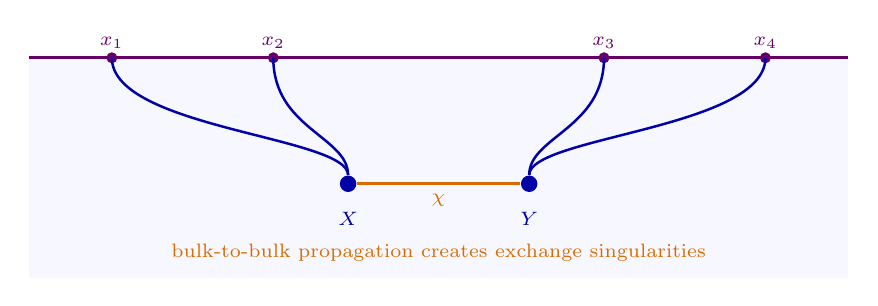
\begin{tikzpicture}[x=1cm,y=1cm,every node/.style={font=\scriptsize}]
    \tikzset{
      ray/.style={blue!65!black,line width=0.9pt},
      internal/.style={orange!85!black,line width=1.0pt},
      boundary/.style={violet!80!black,line width=1.1pt},
      dot/.style={circle,fill=blue!65!black,inner sep=2.1pt}
    }
    \fill[blue!3] (-5.2,-1.45) rectangle (5.2,1.35);
    \draw[boundary] (-5.2,1.35)--(5.2,1.35);
    \foreach \x/\lab in {-4.15/{1},-2.10/{2},2.10/{3},4.15/{4}} {
      \fill[violet!80!black] (\x,1.35) circle (2pt);
      \node[violet!80!black,above] at (\x,1.35) {\(x_{\lab}\)};
    }
    \node[dot] (x) at (-1.15,-0.25) {};
    \node[dot] (y) at (1.15,-0.25) {};
    \draw[internal] (x)--(y) node[midway,below] {\(\chi\)};
    \foreach \a in {-4.15,-2.10} {
      \draw[ray] (\a,1.35) .. controls (\a,0.45) and (-1.15,0.35) .. (x);
    }
    \foreach \a in {2.10,4.15} {
      \draw[ray] (\a,1.35) .. controls (\a,0.45) and (1.15,0.35) .. (y);
    }
    \node[blue!65!black] at (-1.15,-0.70) {\(X\)};
    \node[blue!65!black] at (1.15,-0.70) {\(Y\)};
    \node[orange!85!black,align=center] at (0,-1.12)
      {bulk-to-bulk propagation creates exchange singularities};
  \end{tikzpicture}
  }
  \caption{A four-point exchange Witten diagram contains two integrated bulk
  vertices joined by a bulk-to-bulk propagator.}
  \label{fig:witten-four-point-exchange}
\end{figure}

\section{Mellin Representation}

For scalar primaries, an \(n\)-point function can be represented by a Mellin
integral
\begin{equation}
  \left\langle
    \mathcal O_1(x_1)\cdots\mathcal O_n(x_n)
  \right\rangle
  =
  \int[\dd\delta]\,
  M(\delta_{ij})
  \prod_{1\le i<j\le n}
  \frac{\Gamma(\delta_{ij})}{(x_{ij}^2)^{\delta_{ij}}}.
  \label{eq:mellin-representation-n-point}
\end{equation}
The integration variables \(\delta_{ij}=\delta_{ji}\) satisfy
\begin{equation}
  \delta_{ii}=0,
  \qquad
  \sum_{j\ne i}\delta_{ij}=\Delta_i
  \qquad
  (i=1,\ldots,n).
  \label{eq:mellin-delta-constraints}
\end{equation}
The measure \([\dd\delta]\) denotes integration over a set of independent
complex variables along contours separating the pole families required by OPE
convergence.  The function \(M(\delta_{ij})\) is the Mellin amplitude.

For four points it is common to introduce variables \(s\) and \(t\), with
\[
  s=\Delta_1+\Delta_2-2\delta_{12},
  \qquad
  t=\Delta_1+\Delta_4-2\delta_{14},
  \qquad
  u=\sum_{i=1}^4\Delta_i-s-t.
\]
These variables are Mellin analogues of Mandelstam invariants.  Their
usefulness comes from the fact that local bulk interactions produce simple
analytic behavior in Mellin space.

\section{Contact Terms, Poles, and Locality}

A bulk contact interaction with \(2m\) derivatives gives a Mellin amplitude
that is polynomial of degree \(m\) in the Mellin variables.  In particular, a
non-derivative \(\varphi^4\) interaction produces a constant Mellin
amplitude.  Thus the derivative expansion of a local bulk action becomes a
large-variable polynomial expansion of \(M\).

An exchange diagram produces poles.  If a primary of dimension \(\Delta\) and
spin \(\ell\) is exchanged in the \(12\to34\) channel, then the Mellin
amplitude has pole families of the form
\begin{equation}
  s=\Delta-\ell+2n,
  \qquad
  n=0,1,2,\ldots ,
  \label{eq:mellin-exchange-pole-family}
\end{equation}
with residues that are polynomials of degree \(\ell\) in the transverse
Mellin variables.  The integer \(n\) labels descendants in the exchanged
conformal family.  Double-trace operators arise from the gamma functions in
\eqref{eq:mellin-representation-n-point} and from the full crossing-symmetric
combination of diagrams.

\begin{figure}[H]
  \centering
  \resizebox{0.92\textwidth}{!}{%
  \begin{tikzpicture}[x=1cm,y=1cm,every node/.style={font=\scriptsize}]
    \tikzset{
      arrow/.style={-{Latex[length=2mm]},line width=0.85pt},
      pole/.style={orange!85!black,line width=0.9pt},
      curve/.style={blue!65!black,line width=1.0pt},
      box/.style={draw,rounded corners=4pt,fill=blue!4,inner sep=4pt,align=center}
    }
    \node[box] at (-4.0,1.0) {local contact\\interaction};
    \node[box] at (-4.0,-1.0) {single-particle\\exchange};
    \draw[arrow] (-2.65,1.0)--(-1.35,1.0);
    \draw[arrow] (-2.65,-1.0)--(-1.35,-1.0);
    \begin{scope}[shift={(0.65,1.0)}]
      \draw[->,thick] (-1.15,-0.35)--(1.55,-0.35) node[right] {Mellin variable};
      \draw[->,thick] (-1.05,-0.45)--(-1.05,0.88) node[above] {\(M\)};
      \draw[curve] (-0.85,0.05) .. controls (-0.20,0.28) and (0.65,0.28) .. (1.22,0.06);
      \node[blue!65!black] at (0.25,0.70) {polynomial};
    \end{scope}
    \begin{scope}[shift={(0.65,-1.0)}]
      \draw[->,thick] (-1.15,-0.35)--(1.55,-0.35) node[right] {\(s\)};
      \draw[->,thick] (-1.05,-0.45)--(-1.05,0.88) node[above] {\(M\)};
      \foreach \x/\lab in {-0.55/{\Delta-\ell},0.10/{+2},0.75/{+4}} {
        \draw[pole] (\x,-0.35)--(\x,0.62);
        \node[orange!85!black,below] at (\x,-0.35) {\(\lab\)};
      }
      \node[orange!85!black] at (0.48,0.80) {pole family};
    \end{scope}
    \node[green!45!black,align=center] at (4.0,0)
      {bulk locality becomes\\controlled Mellin analyticity};
    \draw[arrow,green!45!black] (2.25,0)--(3.15,0);
  \end{tikzpicture}
  }
  \caption{In Mellin space, contact interactions give polynomials, while
  exchange diagrams give pole families whose locations are fixed by exchanged
  conformal dimensions.}
  \label{fig:mellin-polynomial-and-poles}
\end{figure}

\section{Crossing in Mellin Space}

Crossing symmetry acts by permuting the external labels and hence by
permuting the constrained variables \(\delta_{ij}\).  For identical scalar
operators, the Mellin amplitude is symmetric under the corresponding
permutation group:
\[
  M(\delta_{ij})=M(\delta_{\sigma(i)\sigma(j)})
  \qquad
  \sigma\in S_n.
\]
This symmetry couples the pole expansion in different OPE channels.  A pole
associated with one exchanged single-trace primary must be accompanied by the
contact terms and crossed-channel structures that make the full correlator
single valued and crossing symmetric.

The Mellin representation is therefore a bridge between two descriptions of
the same data.  On the CFT side, poles and residues encode OPE coefficients,
dimensions, and descendants.  On the bulk side, the same analytic structure is
computed by local vertices, propagating fields, and the derivative expansion
of an effective action in \(\mathrm{AdS}_{D+1}\).
